\documentclass{article}
% translate with >> pdflatex -shell-escape <file>

% This file is used as unit test for pgfplots, copyright by Christian Feuersaenger.
% 
% See
%   http://pgfplots.sourceforge.net/pgfplots.pdf
% for pgfplots.
%
% Any required input files (for <plot table> or <plot file> or the table package) can be downloaded
% at
% http://www.ctan.org/tex-archive/graphics/pgf/contrib/pgfplots/doc/latex/
% and
% http://www.ctan.org/tex-archive/graphics/pgf/contrib/pgfplots/doc/latex/plotdata/

\usepackage{pgfplots}
\pgfplotsset{compat=1.4}

\pagestyle{empty}

\begin{document}
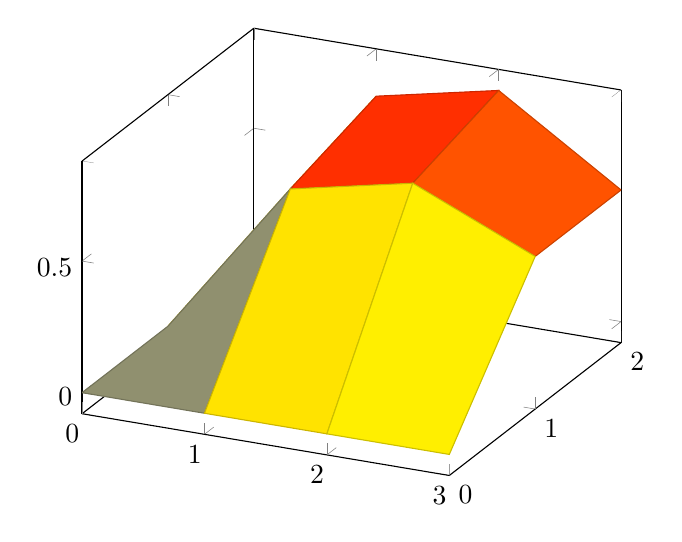
\begin{tikzpicture}
	\begin{axis}
		\addplot3[surf] table[y=col2,z expr=\thisrow{col3}*1,row sep=crcr] {
			col1 col2 col3\\
			 0 0 0\\
			 1 0 0\\
			 2 0 0\\
			 3 0 0 \\
\\
			 0 1 0\\
			 1 1 0.6\\
			 2 1 0.7\\
			 3 1 0.5 \\
\\
			 0 2 0\\
			 1 2 0.7\\
			 2 2 0.8\\
			 3 2 0.5 \\
		};
	\end{axis}
\end{tikzpicture}
\end{document}
